\documentclass[11pt,a4paper]{article}
\usepackage{bbm,amsthm,amsfonts,amssymb,amsmath,latexsym,epic,eepic}
\usepackage{marvosym,graphicx,fancyhdr,bbm}
\usepackage{graphicx}
\usepackage{gensymb}
\usepackage{url}
\usepackage{color}
\usepackage[rflt]{floatflt}
\usepackage{colortbl}
\usepackage{subcaption}
\usepackage{url}
\usepackage[vlined, ruled, boxed]{algorithm2e}
\definecolor{Grey}{rgb}{0.5,0.5,0.5}
\definecolor{Red}{rgb}{1.0,0.0,0.0}
\renewcommand{\figurename}{Abbildung}
\usepackage{typearea}
\areaset{156mm}{235mm}
%\setlength{\parskip}{5pt plus 2pt minus 1pt}
\setlength{\parindent}{0pt}

% use \M for matrices and \V for vectors in math mode
\newcommand{\M}[1]{\mathbf{#1}}
\newcommand{\V}[1]{\mathbf{#1}}
\newcommand{\norm}[1]{\left | \left | #1 \right | \right |}
\newcommand{\RR}{\mathbbm{R}}        % set of real numbers


\renewcommand\floatpagefraction{0.8}
\renewcommand\topfraction{1}
\renewcommand\bottomfraction{0.9}
\renewcommand\textfraction{0.0}
%\def\dbltopfraction{1.0}
%\def\bottomfraction{1.0}
%\def\dblfloatpagefraction{0.8}


\makeatletter
\renewenvironment{thebibliography}[1]
     {\section*{\refname}%
      \@mkboth{\MakeUppercase\refname}{\MakeUppercase\refname}%
	 \parsep0mm
	 \itemsep0mm
	 %\labelsep0mm
	 %\itemindent0mm
      \list{\@biblabel{\@arabic\c@enumiv}}%
           {\settowidth\labelwidth{\@biblabel{#1}}%
            \leftmargin\labelwidth
            \advance\leftmargin\labelsep
            \@openbib@code
            \usecounter{enumiv}%
            \let\p@enumiv\@empty
            \renewcommand\theenumiv{\@arabic\c@enumiv}}%
      \sloppy
      \clubpenalty4000
      \@clubpenalty \clubpenalty
      \widowpenalty4000%
      \sfcode`\.\@m}
     {\def\@noitemerr
       {\@latex@warning{Empty `thebibliography' environment}}%
      \endlist}
\renewcommand\newblock{\hskip .11em\@plus.33em\@minus.07em}
\let\@openbib@code\@empty
\makeatother



\begin{document}\sloppy

\title{\Large\bf Test von Algorithmen zur Lokalisation, Kartierung und Pfadverfolgung \footnotetext{Diese Arbeit ist Bestandteil des Praktikums zur Mess- und Regelungstechnik}}

\author{Kai Hofmann und Barbara Fischbach\\
  Robotik und Telematik \\
  Universit\"at W\"urzburg\\
  Am Hubland, D-97074 W\"urzburg\\
{\small \texttt{barbara.fischbach@uni-wuerzburg.de}}\\
{\small \texttt{kai.hofmann@uni-wuerzburg.de}}}

\date{}



\maketitle


\newpage

\twocolumn

\section*{Abstract}

	\addcontentsline{toc}{section}{Abstract}

	\textbf{Die autononome Fortbewegung von Fahrzeugen spielt heutzutage eine immer gr\"o\ss{}ere Rolle. Dazu werden verschiedene Algorithmen, zur Lokalisierung, Kartierung und Pfadverfolgung ben\"otigt. Diese werden auf einer realen Roboter-Platform mit Differentialantrieb implementiert und auf Funktion und Genauigkeit getestet. Die Versuche zeigen dass Pfadverfolgung mit dem \textit{Giovanni Controller} m\"oglich ist. }

\section{Einleitung}
	Selbstfahrende Fahrzeuge sind ein gro{\ss}es Thema der Zukunft. Damit diese zuverl\"assig und sicher fahren k\"onnen braucht es gute Algorithmen in verschiedenen Bereichen. Wie gut bestehende Ans\"atze funktionieren und wo deren Schw\"achen sind wird in diesem Paper anhand einer Roboter-Plattform mit Laserscanner untersucht. 

	Zur Lokalisierung in einer zuvor kartierten Umgebung kann der \textit{Adaptive Monte Carlo Localization}-Algorithmus, von Dieter Fox im Paper \textit{KLD-Sampling: Adaptive Particle Filters} \cite{amclPaper} vorgestellt, verwendet werden. 
	
	Die daf\"ur ben\"otigte Karte kann mit dem \textit{SLAM-Gmapping}-Algorithmus von Giorgio Grisetti generiert werden. Der Algorithmus wird im Paper \textit{Improved Techniques for Grid Mapping
	with Rao-Blackwellized Particle Filters} \cite{Gmapping} besprochen. Dieser l\"ost dass Problem der gleichzeitigen Lokalisation und Kartierung durch die Nutzung des Laserscanners schon bei der Lokalisation und nicht erst bei der Kartiertung. 
	
	Mit einer guten Lokalisation ist es m\"oglich einem Pfad zu folgen. Daf\"ur hat Giovanni Indiveri einen Algorithmus, im Paper \textit{SWITCHING
	LINEAR PATH FOLLOWING FOR
	BOUNDED CURVATURE CAR-LIKE
	VEHICLES} \cite{Giovanni} beschrieben, entwickelt. 

	Die drei Algorithmen werden im Abschnitt 2 genauer erkl\"art. Im Abschnitt 3 folgt eine kurze Beschreibung unserer Testplattform und dem verwendeten \textit{Robot Operating System}. Abschlie{\ss}en folgt eine Vorstellung und Diskussion der Test-Ergebnisse im Abschnitt 4.
  

\section{Algorithmen}

\subsection{Lokalisation}
\subsubsection{Odometrie}
{
	Die Odometrie ist eine einfache M\"oglichkeit der relativen Positionsbestimmung und bildet die Grundlage f\"ur anspruchsvollere Algorithmen wie \textit{AMCL}. Dabei wird aus der vorher bekannten Position des Roboters und der vermuteten zur\"uckgelegten Weg-strecke die neue Position berechnet. Die Wegstrecke wird \"uber die Steuerungsbefehle und ein Modell des Roboters berechnet. Da es kein weiteres Feedback \"uber die Position gibt, ist dies ein \textit{Open loop}. 
}
\subsubsection{Adaptive Monte Carlo Localization \cite{mclWiki} \cite{amclPaper}} 
{
	Im folgenden als AMCL abgek\"urzt, ist ein Algorithmus der mit Hilfe eines Partikelfilters die Position eines Roboters bestimmt. Dazu wird eine Karte der Umgebung ben\"otigt. Da die Pose zu Beginn nicht bekannt ist, stellt der Roboter Hypothesen dar\"uber auf der Karte an, verteilt also die Partikel \"uber den Zustandsraum. Die anf\"angliche Verteilung auf der Karte kann verschieden sein. Es ist zum Beispiel m\"oglich diese  gleichm\"a{\ss}ig über die ganze Karte zu verteilen. 
	Bei der von den Autoren verwendeten Implementation ist sie Gau{\ss}-verteilt um eine gegebene anf\"angliche Pose, siehe Abbildung ~\ref{fig:initalParticleDistribution}. \begin{figure}[h]
		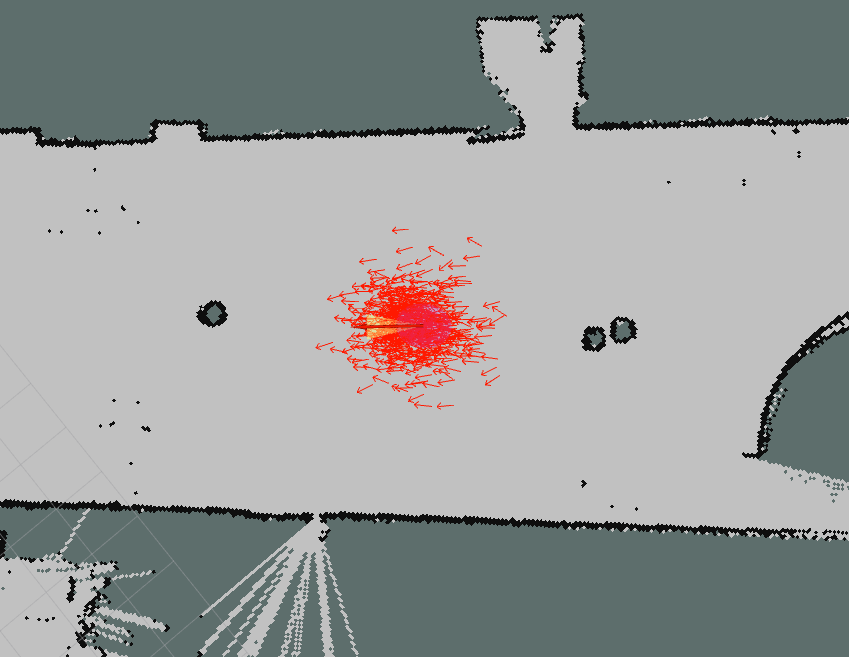
\includegraphics[width=\linewidth]{pictures/initial_distribution.jpg}
		\caption{Partikelverteilung in Anfangspose \label{fig:initalParticleDistribution}}
	\end{figure}
	\newpage
	Ist der Roboter tats\"achlich an einem anderen Ort, so hat er keine Chance sich zu lokalisieren. 
	
	Die Hypothesen kann man sich als virtuelle Roboter auf der Karte vorstellen. F\"ahrt der reale Roboter, so fahren auch die virtuellen Roboter, mit den gleichen Steuerungsbefehlen. Die realen Sensorwerte werden mit denen der virtuellen Robotern verglichen. Die virtuellen Roboter gewinnen ihre Sensormesswerte durch die Karte. Als reale Sensormesswerte werden die Messungen des Laserscanners verwendet. 
	
	Je unstimmiger die Daten des virtuellen Roboters sind, desto unwahrscheinlicher ist die Hypothese, dass der Reale sich dort befindet. Daher werden jene Partikel gel\"oscht. Im Bereich der wahrscheinlichen Hypothesen, werden neue Partikel/Hypothesen erzeugt.
	
\begin{figure}[h]
	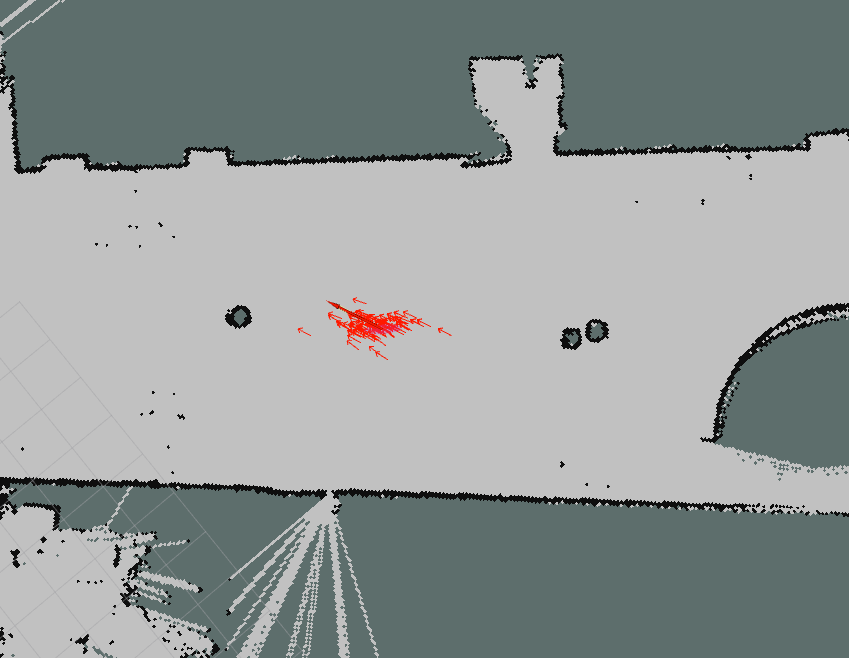
\includegraphics[width=\linewidth]{pictures/drive_little.jpg}
	\caption{Partikelverteilung nach kurzer Neuorientrierung durch Bewegung. Man erkennt die Partikel sind konzentrierter}
\end{figure}
		
	Der virtuelle Roboter  mit besten den \"Ubereinstimmungen, ist die beste Estimation der Pose.
	Je n\"aher die wahrscheinliche Hypothesen bei einander liegen, desto sicherer ist der Roboter sich seiner Pose. In diesem Fall kann die Anzahl der Partikel reduziert werden um Ressource, wie Speicherplatz zu sparen. Daher das \textit{Adaptive} aus \textit{AMCL}.
}
\newpage
\subsection{Kartierung mit gmapping  \cite{Gmapping}}
{
	Zur Lokalisation braucht der Roboter eine Karte. Eine unbekannte Umgebung wird dabei mit den Daten eines Laserscanners und den aktuellen Posedaten erfasst und von dem Algorithmus GMapping verarbeitet.
	
	Die Idee des  \textit{Grid}Mappings ist, die ungenauen Sensordaten einer Umgebung, auf einer 2D-Karte in bin\"aren Zufallsvariablen darzustellen. Dabei wird die Karte in Gitter unterteilt, in dem jedes Quadrat mit einer Wahrscheinlichkeit aussagt, ob es belegt ist oder nicht. Die Variablen stellen also Objekte in der Umgebung dar. Algorithmen, wie AMCL, werten die Zufallsvariablen aus.  
	
	Die Herausforderung liegt bei der Kartierung in der gleichzeitigen Lokalisierung und Kartierung, dem \textit{simultaneous localization and mapping} Problem kurz \textit{SLAM}. Denn beide bedingen sich gegenseitig. Um  zwei Laserscans zu einer Karte zusammenzuf\"ugen, m\"ussen die relativen Posen der Aufnahmen bekannt sein. Also ein Lokalisierungsproblem. Und um sich mit dem Laserscanner zu lokalisieren, ben\"otigt man wiederum Kartendaten. \\
    
    Ein einfacher Ansatz ist die Odometrie zu verwenden um die relativen Posen zwischen zwei Aufnahmen des Laserscanners zu bestimmen. Die resultierenden Karten sind nicht nutzbar. Daher werden bei der Bestimmung der relativen Posen schon die Laserscandaten verwendet. Diese Technik wird \textit{Scanmatching} genannt. Die Information über die relativen Posen von \textit{Scanmatching} und Odometrie wird fusioniert um eine bestm\"oliche Sch\"atzung der Pose zu gewinnen.

\subsection{Pfadverfolgung mit Giovanni-Controller}


\begin{figure}[h]
	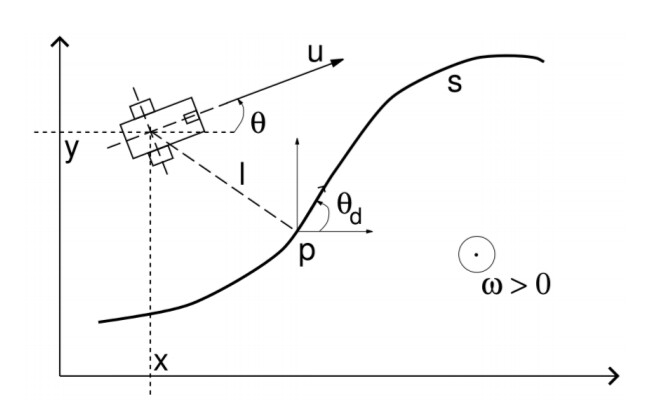
\includegraphics[width=\linewidth]{pictures/Pfadverfolgung.JPG}
	\caption{Modell der Pfadverfolgung}
\end{figure}

	Der nicht-lineare Regler des Giovanni Indiveri und der Maria L. Corradini\cite{Giovanni} wird zur Pfadverfolgung verwendet. Er basiert auf der Arbeit von Canudas de Wit et al. \cite{Canudas} und ist um eine Funktion erweitert, die den  minimalen Wendekreis, wie auch die maximale Geschwindigkeit des Roboters ber\"ucksichtigt. Die Implementierung garantiert nach Lyapunov, f\"ur einen beschr\"ankten, nicht-linearen Pfad, asymptotische Konvergenz und asymptotisch stabile Fehlerdynamik. Schrittweise neue Berechnungen der Reglerparameter f\"uhren zu einer schnelleren Konvergenz. Hierzu verwendet der Algorithmus eine orthogonale Projektion auf den Roboter selbst. Das Modell in Abbildung 5 stellt den abzufahrenden Pfad dar. Dabei ist der Winkel zwischen der x-Achse und der L\"angsachse des Roboters $\theta$ und $\theta_{d}$
beschreibt den Winkel einer Tangente an den Pfad zur 
x-Achse. Die Differenz 
\begin{equation}
\tilde{\theta} = \theta -\theta_{d}
\end{equation}
beschreibt den Winkel der Fahrtrichtung des Roboters und der Tangente an einem Pfadpunkt p. Der Abstand zwischen der orthogonalen Projektion des Roboters auf den Pfad und des Rotationszentrums des Roboters ist gegeben durch l.
Der Pfad wird zur Vereinfachungen in lineare Teilschnitte gen\"ahert, wodurch sich die Gleichungen vereinfachen. Die Formel f\"ur die Winkelgeschwindigkeit $\omega$ mit der linearen Geschwindigkeit u des Roboters


\begin{equation}
\omega=  \frac{u \kappa(s) cos(\tilde{\theta})}{1-l \kappa(s)}-h u l  \frac{sin(\tilde{\theta})}{\tilde{\theta}}-\gamma\tilde{\theta} :h\gamma > 0
\end{equation}\\

vereinfacht sich im linearen Fall $\kappa(s)=0$ zu \\

\begin{equation}
\omega= -h u y  \frac{sin(\theta)}{\theta}-\gamma\theta :h\gamma > 0
\end{equation}\\



	Durch Koordinatentransformation, dient die x-Achse als die Fahrtrichtung des Robotors  und y (der Roboter-Pfad-Abstand) \"ubernimmt die Rolle des l. Der Winkel Theta wird durch das \"ubereinanderlegen zu null.


\section{Test-Plattform}
\subsection{ROS}

F\"ur die Implementierung und Tests der Algorithmen wird das \textit{Robot Operating System}, kurz ROS genutzt. Es ist kein Betriebssystem im eigentlichen Sinne, sondern ein Framework. Es erm\"oglicht Hardware-Abstraktion, Paket-Management und stellt eine Middleware, bereit mit der verschiedene Prozesse kommunizieren k\"onnen. \cite{rosWiki}

\begin{figure}[h]
	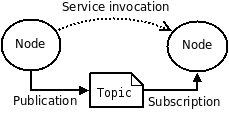
\includegraphics[width=\linewidth]{pictures/ROS_basic_concepts.png}
	\caption{Kommunikation zwischen Nodes \label{fig:rosNodes}}
\end{figure}

Die ROS-Software ist in sogenannten Nodes organisiert, welche die eigentlichen Berechnungen durchf\"uhren. Der ROS-Master hilft den Nodes sich zu finden und eine Verbindung aufzubauen. Die Kommunikation zwischen den Nodes erfolgt dann direkt untereinander \"uber ein ROS spezifisches Protokoll dass auf TCP/IP aufsetzt. Nodes k\"onnen auf Topics ver\"offentlichen und diese abonnieren, siehe dazu Abbildung ~\ref{fig:rosNodes}. \cite{rosConcepts}


Durch die Nodes k\"onnen Funktionalit\"aten wie Planung, Pfadverfolgung, Sensorik, etc getrennt werden. Au{\ss}erdem k\"onnen so einfach Nodes anderer Leuten genutzt werden. Dies erm\"oglicht es in kurzer Zeit eine Plattform zum Testen der Algorithmen aufzubauen, und ohne gro{\ss}en Aufwand Algorithmen durch Nodes zu implementieren. ROS-Nodes k\"onnen in C++ oder Python geschrieben werden.

\subsection{Hardware}
 
Zur Verf\"ugung stehen drei Roboter mit Differentialantrieb. Zwei vom Typ Volksbot mit Motor Controller VMC, sowie ein Robotersystem mit dem EPOS2 Motor Controller von \textit{maxon motor control}. Der VMC \cite{Volksbot} wird mittels serieller Schnittstelle mit dem Steuerrechner verbunden. Neben der Motoransteuerung k\"onnen Geschwindigkeit und Strom mittels eines PID-Reglers kontrolliert werden. 
Differentialantrieb ist ein Antrieb zweier unabh\"angiger R\"ader, die sich auf einer starren Achse befinden. Werden die R\"ader mit unterschiedlicher aber nicht nivellierender Geschwindigkeit angetrieben, f\"ahrt der Roboter eine Kurve. Sind die Geschwindigkeiten dagegen gleich, ist die resultierende Spur gerade.
Da sich die Roboter im Aufbau und in der Betriebsweise gleichen, k\"onnen die Algorithmen auf allen gleich gut getestet werden.

Bei allen verwendeten Robotern ist an der Front ein SICK LMS100 Laserscanner auf einer H\"ohe von etwa 35 cm montiert. Dieser hat einen Arbeitsbereich von 270\degree  und eine Reichweite von bis zu 20 Metern.\cite{lms} 
 
ROS l\"auft auf einem handels\"ublichen Notebook, das auf den Roboter gestellt wird und \"uber LAN und USB mit dem Roboter verbunden ist. 
 

\begin{figure}[h]
	\centering
	{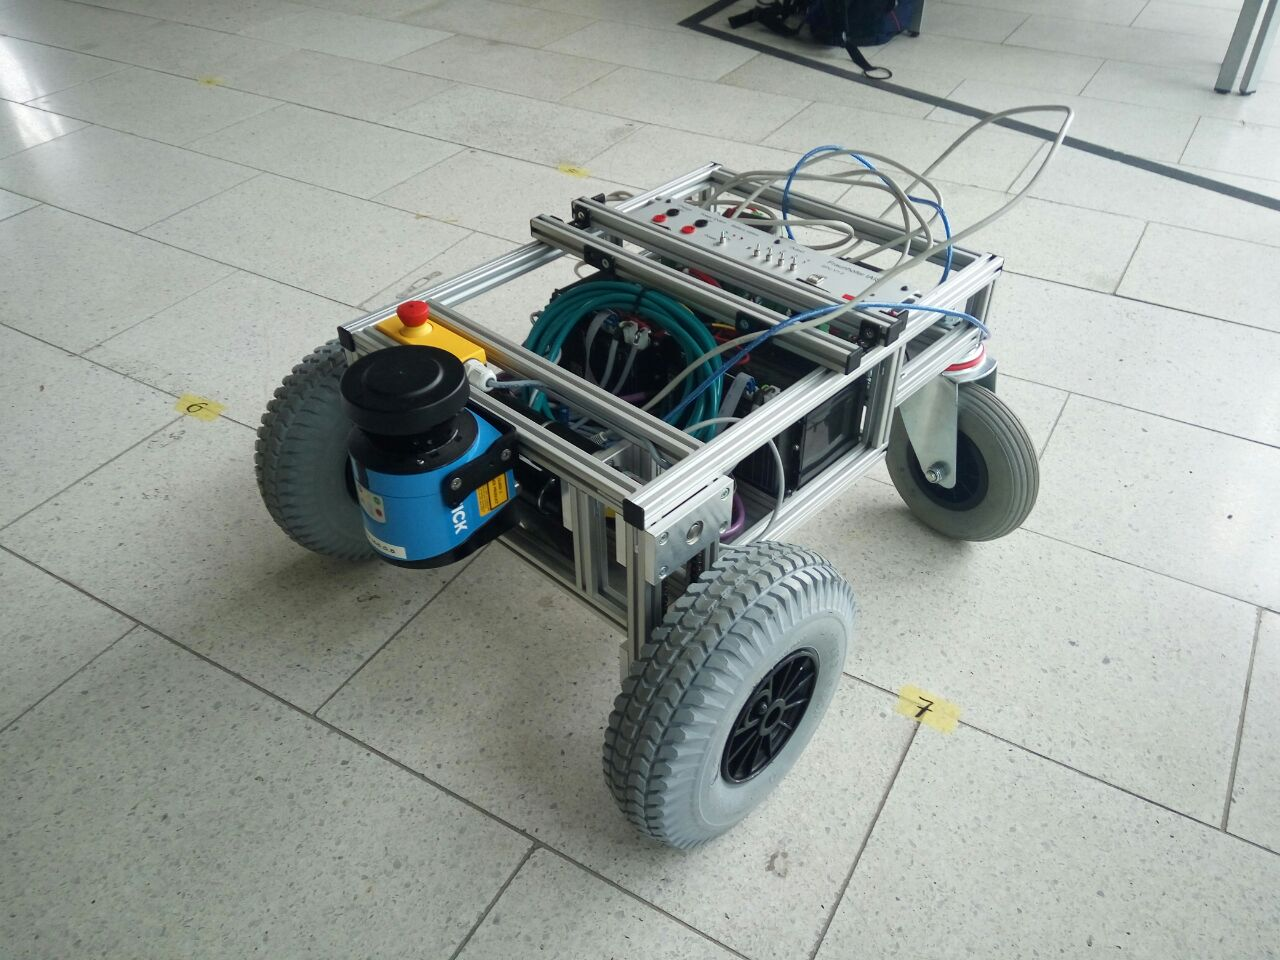
\includegraphics[trim= 2cm 2cm 2cm 2cm, clip=true,width=\linewidth]{pictures/robot.jpg}}
	\caption{\textit{Ute} - Einer der verwendeten Roboter}
\end{figure}


\subsection{Genutzte Nodes}
{

	\begin{figure*}[h]
		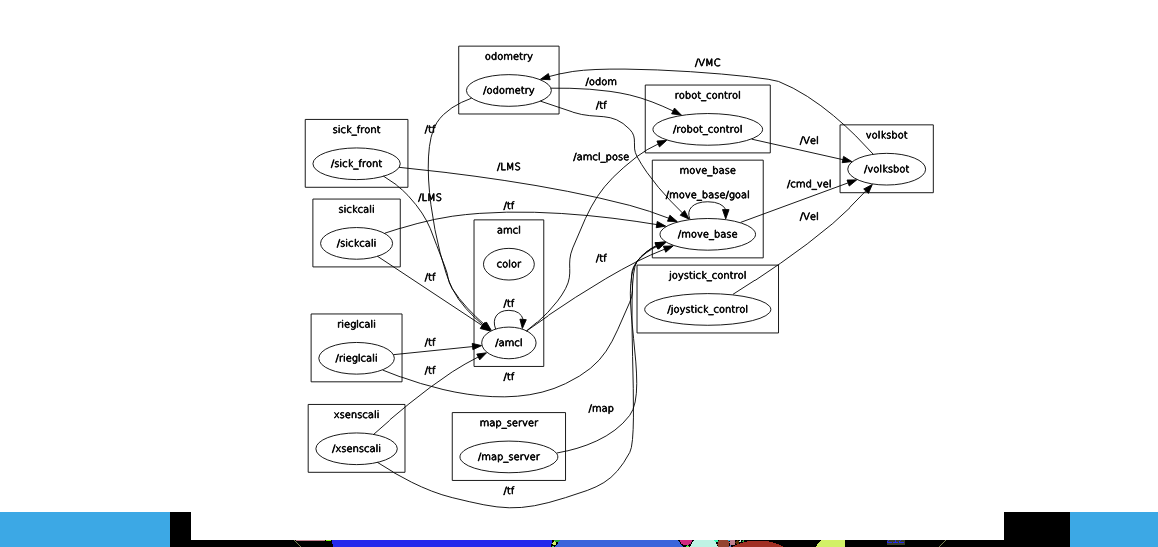
\includegraphics[trim=9cm 1cm 7cm 1cm , clip= true,width=\textwidth]{pictures/node_graph.png}
		\caption{Vernetzung der \textit{Nodes} im Testaufbau \label{fig:nodes}}
	\end{figure*}
	Die verwendete Software ist in \textit{ROS Nodes} organisiert. Deren grobe Verbindungen untereinander wird im Folgenden skizziert, f\"ur den Fall der Pfadverfolgung mit AMCL mit zuvor bekannter Karte beschrieben. Siehe dazu Abbildung ~\ref{fig:nodes}. 
	\\
	Zun\"achst gibt es Nodes die f\"ur die Sensoren zust\"andig sind, sie abstrahieren die Hardware wie den Laserscanner und die Odometrie (\textit{sick\_front} und \textit{odometry}). Deren Daten verwendet die \textit{AMCL Node} f\"ur die Lokalisierung. Die Pose wird dann zur \textit{robot\_control-Node}, der f\"ur die Pfadverfolgung zust\"andig ist weitergeleitet. Dieser leitet dann Information über die ben\"otigten R\"adergeschwindigkeiten and die \textit{Node Volksbot} weiter, welcher die Motoren ansteuert.
	
} 

\section{Test der Algorithmen} 
\subsection{Odometrie und AMCL im Vergleich}




Um die Lokalisation durch AMCL und Odometrie miteinander zu vergleichen f\"ahrt der Roboter einen "Acht"-f\"ormigen Pfad ab. Die Steuerung erfolgt manuell \"uber einen Joystick und wird zweimal in verschiedenen Geschwindigkeiten durchgef\"uhrt. Siehe dazu Abbildung ~\ref{fig:odo_amcl}. Bei der Erstellung dieser Grafik gab es ein Problem: AMCL und Odometrie sollten beide im Ursprung starten, also bei der Pose (0$|$0$|$0). Denn so ist ihre Darstellung vergleichbarer. Damit AMCL jedoch korrekt arbeitet muss der Roboter erst ein Stück weit fahren. Dann ist jedoch die Odometrie nicht mehr bei (0$|$0$|$0). Um dieses Problem zu umgehen werden die Koordinatensysteme vor dem plotten so transformiert dass der Roboter, in der Darstellung immer bei (0$|$0$|$0) startet. Dies \"andert nichts an Geomtetrie und Abst\"anden.    


\begin{figure}[h]
	\centering
	\subcaptionbox{Mit einer Geschwindigkeit $\leq$ 0.8m/s}{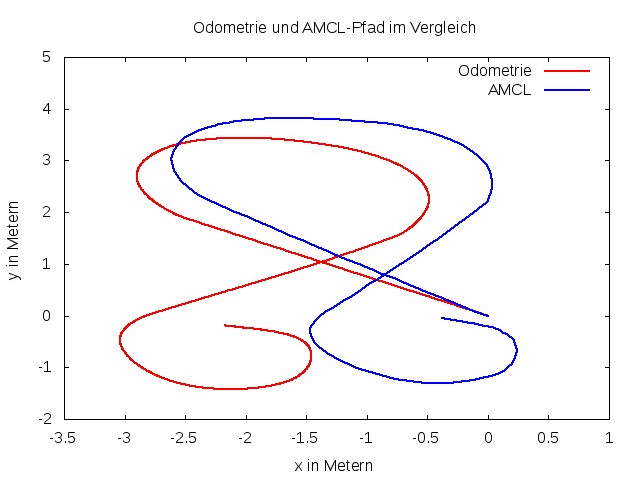
\includegraphics[width=\linewidth]{pictures/odo_amcl_comparision_slow.jpg}}\par\medskip
	\centering
	\subcaptionbox{Mit einer Geschwindigkeit $\geq$ 3.3m/s}{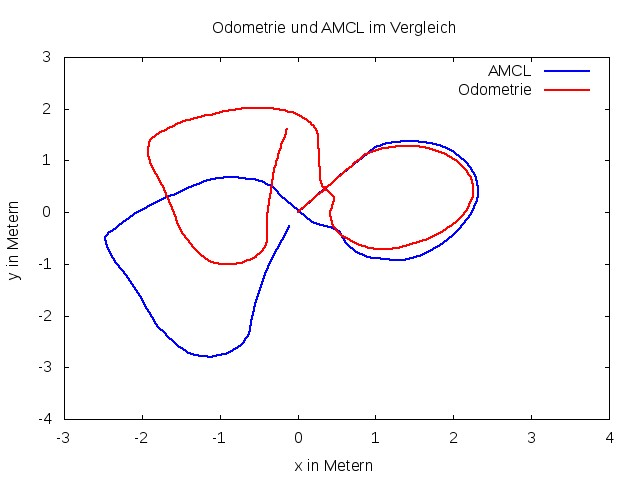
\includegraphics[width=\linewidth]{pictures/odo_amcl_comparision_fast.jpg}}\par\medskip
	\caption{ Odometrie und AMCL im Vergleich. \label{fig:odo_amcl}}
\end{figure}

Im Experiment, siehe Abbildung ~\ref{fig:odo_amcl}, zeichnet sich bereits zu Beginn der Durchf\"uhrung ab, dass der Odometriepfad fehlerhaft ist. Jedoch unter der Annahme dass \textit{AMCL} der Wahrheit entspricht. Diese Annahme wird dadurch gestützt dass \textit{AMCL} "behauptet" dass der Roboter zu seiner Startpose zurück kehrt und dies von den Autoren auch so beobachtet wurde.  
Eine belastbarere Aussage kann man treffen wenn der Roboter zu seinem Startpunkt zurückgekehrt ist, denn dieser wurde auf $\leq$ 5 cm genau angefahren. Bei der Odometrie summieren sich die Fehler auf und die Zielpose weicht bis zu 2 m von der Startpose ab. 
Der AMCL Pfad dagegen, kehrt bis auf wenige Zentimeter zur Startpose zur\"uck. Bei der Orientierung macht AMCL Fehler die für Menschen direkt ersichtlich sind, siehe dazu Abbildung ~\ref{fig:amclFails}.

 Zus\"atzlich muss in diesem Versuch die menschliche Ungenauigkeit, vorallem beim schneller abgefahrenen Pfad, wie ungenaues Augenma{\ss} und Steuerungsschwierigkeiten, beachtet werden. Aus dem Vergleich ist ersichtlich, dass der Fehler bei AMCL auch in der Distanz, also bei langen Pfaden, nicht gr\"o{\ss}er ist, als er auch bei k\"urzer w\"are, w\"ahrend bei der Odometrie bei langer Laufzeit die Qualit\"at stetig abnimmt. 

Die schlechteren Ergebnisse der Odometrie k\"onnen wie folgt erkl\"art werden. Mit wachsender Entfernung nehmen auch Fehler durch zum Beispiel unterschiedliche Dr\"ucke in den Reifen oder eine verst\"arkte Reibung oder Unebenheiten auf anderem Gel\"ande zu. Weitere Fehlerquelle sind h\"oheren Geschwindigkeiten und engeren Kurven, dort neigen die R\"ader zum Durchdrehen und Wegrutschen. 	



Von der Lokalisierungsperformance abgesehen gibt es weitere Vor- und Nachteile. So ben\"otigt AMCL eine Karte um funktionieren zu k\"onnen. Au{\ss}erdem ist der Rechenaufwand bei AMCL h\"oher und daher ist AMCL seltener vef\"ugbar. 


\begin{figure}[h]
	\centering
	{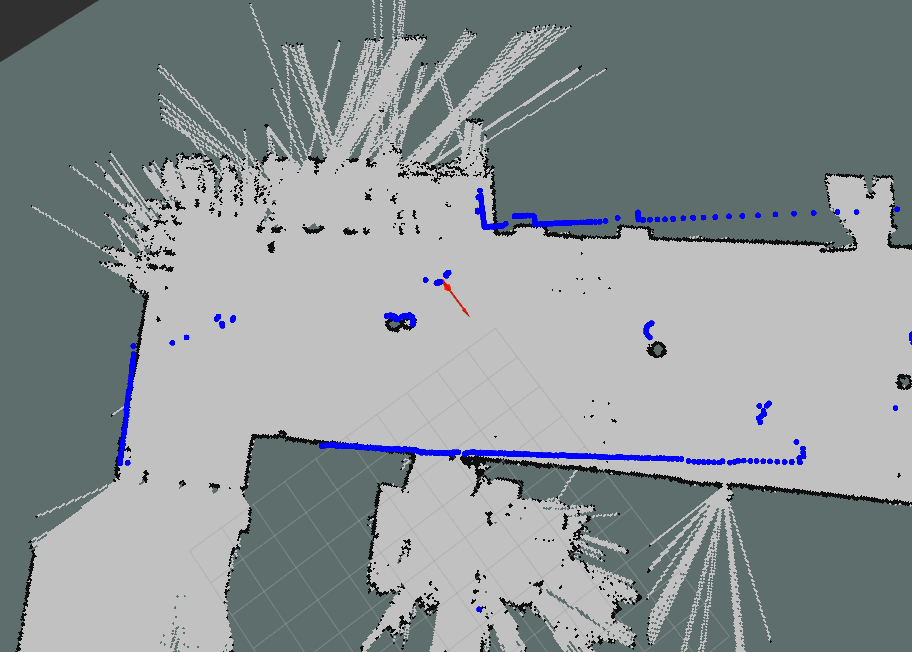
\includegraphics[width=\linewidth]{pictures/amcl_fail.png}}
	\caption{ Auch bei \textit{AMCL} gibt es Abweichungen \label{fig:amclFails}}
\end{figure}




\subsection{Test von Gmapping}
{
	Das Untergeschoss des Informatikinstituts W\"urzburg ist mit einem Frauenhofer-Roboter, der mit einem Sick LMS100 Laserscanner ausgestattet ist, in einer 2D-Karte kartiert.  Um diese Karte korrekt aufzunehmen, werden nur zehn Partikel ben\"otigt. Die Aufnahme ist bis auf einen 1 cm genau und zeigt keine signifikanten Fehler. Bewegte Objekte wie Menschen werden erkannt und nicht in der Karte verzeichnet. Dagegen sorgt helles Licht, das durch die Fensterfronten scheint, f\"ur eine Ungenauigkeit und kann nicht als klare Begrenzung festgestellt werden. F\"ur klare Linie wie W\"ande ist es wichtig, das Gel\"ande mit einem Geschwindgkeitslimit von 2 km/h (halbe Schrittgeschwindigkeit) abzufahren.  
	
	\begin{figure}[h]
		\centering
		\subcaptionbox{fehlerhafte Karte}{
			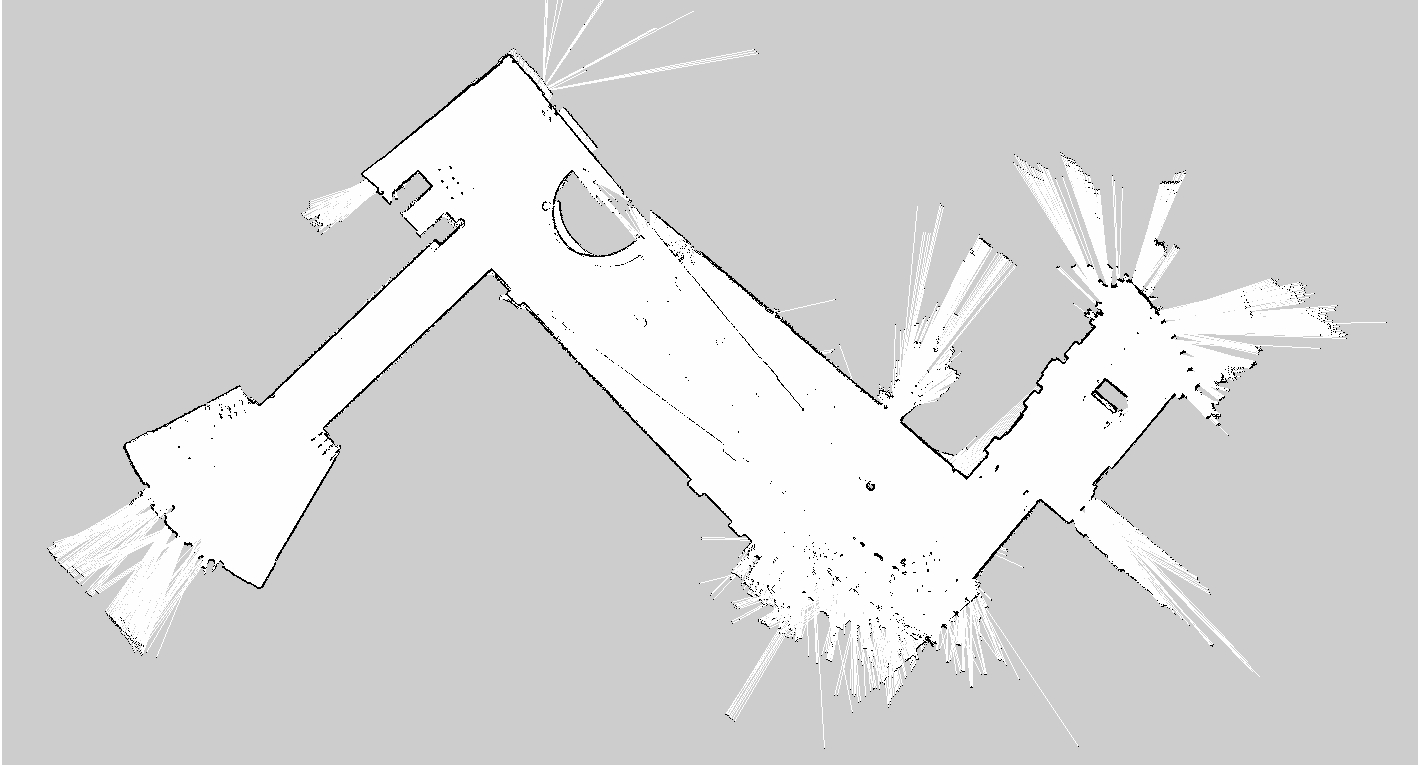
\includegraphics[width=0.45\textwidth]{pictures/firstMap.jpeg}}
		\subcaptionbox{korrekte Karte}{
			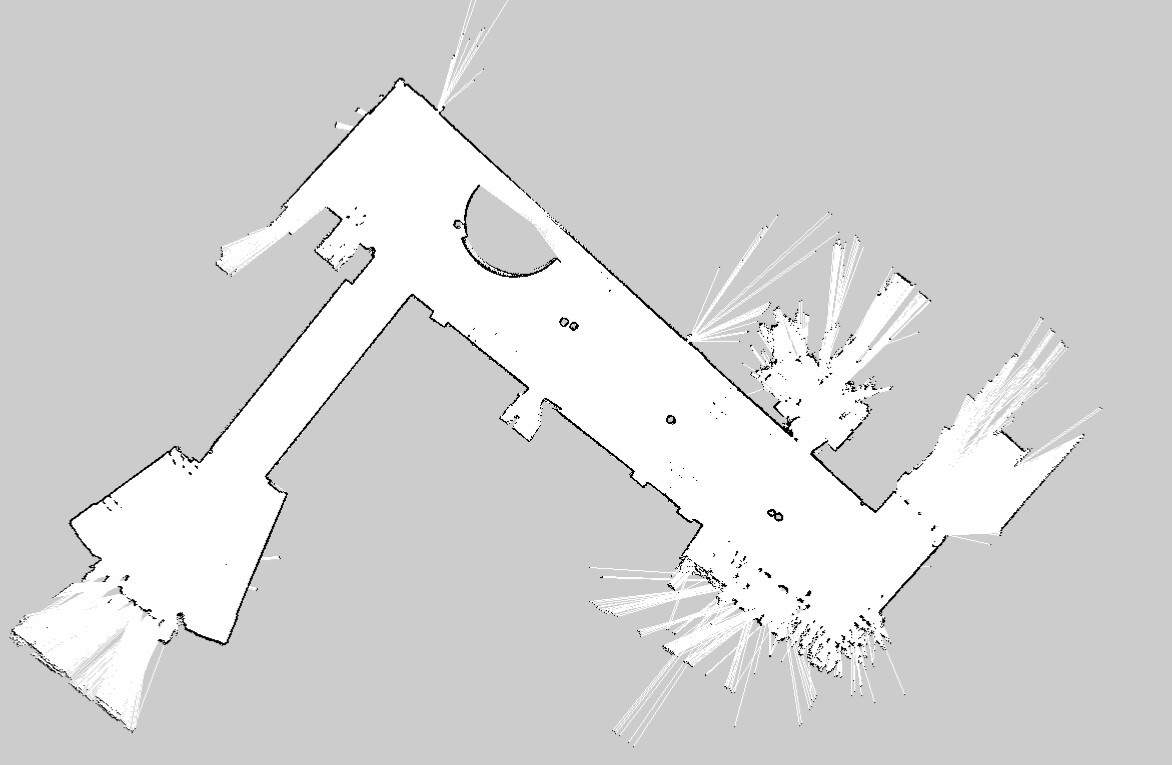
\includegraphics[width=0.45\textwidth]{pictures/correctMap.JPG}}
		\caption{Karten aufgezeichnet mit Gmapping}
	\end{figure}
	
	
	Deutliche Unterschiede sind in den Karten von Abbildung 4 zu erkennen. Bild (a) zeigt eine Karte, die im ersten Versuch aufgenommen ist und aus Unwissenheit mit zu hoher Geschwindigkeit und nicht oft genug abgefahren ist. Im Vergleich dazu ist die Karte (b) durch langsameres und stetigeres Abfahren detailgetreuer und hat klare Linien.
	
		
}




\subsection{Test und von \texttt{gio\_path}}


Zun\"achst wird die Pfadverfolgung simuliert, um den Algorithmus auf theoretische Funktion zu testen. Der Robotersimulator wird als ROS-Node implementiert und soll vorgebene Pfaddateien abfahren.


\begin{figure}[h]
	\subcaptionbox{Verfolgung eines spiralf\"ormigen Pfades\label{fig:simulatedSpiral}}{
		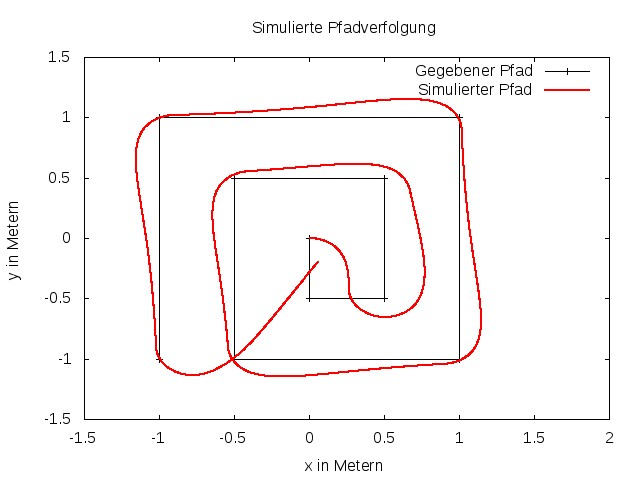
\includegraphics[width=\linewidth]{pictures/simulated_spirale.jpg}
		
	}
	\subcaptionbox{Verfolgung eines Acht-f\"ormigen Pfades}{
		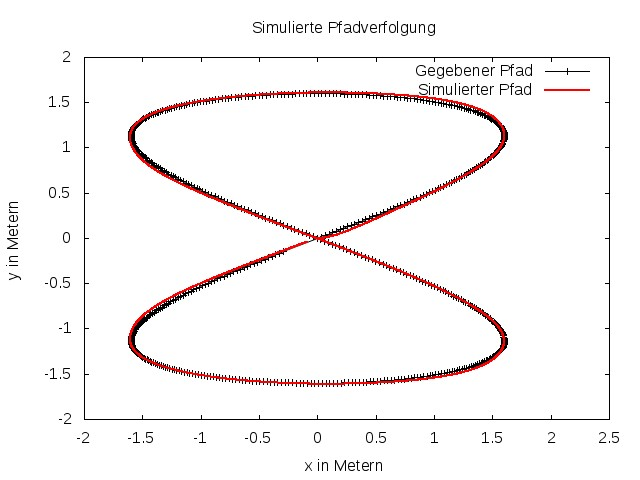
\includegraphics[width=\linewidth]{pictures/simulated_acht.jpg}}
	\caption{Simulierte Pfadverfolgung}

\end{figure}
Es zeigt sich, dass der Giovanni-Controller nicht immer alle Punkte des Pfades perfekt ansteuert, wie in Abbildung ~\ref{fig:simulatedSpiral} zu erkennen.  


\newpage
Um den \texttt{gio\_path} Algorithmus auf einem realen Roboter zu testen, wird erneut eine ROS-Node verwendet. Diese benutzt  \texttt{gio\_path} um einen realen Roboter zu steuern. Der Algorithmus steuert den Roboter wie folgt: 

\begin{algorithm}
	pathDone $\leftarrow$ false\;
	rightSpeed $\leftarrow$ 0.0\;
	leftSpeed $\leftarrow$ 0.0\;
	controller.setPath(pathFile)\;
	\While{!pathDone}{
		controller.setPose(currentPose)\;
		pathDone = controller.getNextState(leftSpeed, rightSpeed)\;
		publishToMotors(leftSpeed, rightSpeed);
	}
\caption{\textit{Giovanni Controller} Implementation}
\end{algorithm}

Die Autoren entscheiden sich als Testpfad eine 12m lange Spirale zu nutzen. Dieser Pfad wird viermal abgefahren, einmal mit Odometrie als Input f\"ur \textit{Giovanni Controller} und einmal mit \textit{AMCL} als Input, jeweils mit erh\"ohter und niedriger Geschwindigkeit.

Da die Autoren leider keine M\"oglichkeit haben die Position des Roboters extern zu verfolgen, wird f\"ur die Analyse der Pfadverfolgung mit Odometrie \textit{AMCL} als "Wahrheit" verwendet.
\newpage
\begin{figure}
	\centering
	\subcaptionbox{niedrige Geschwindigkeit $\approx$ 0,714m/s \label{fig:odoLowSpeed}}{
		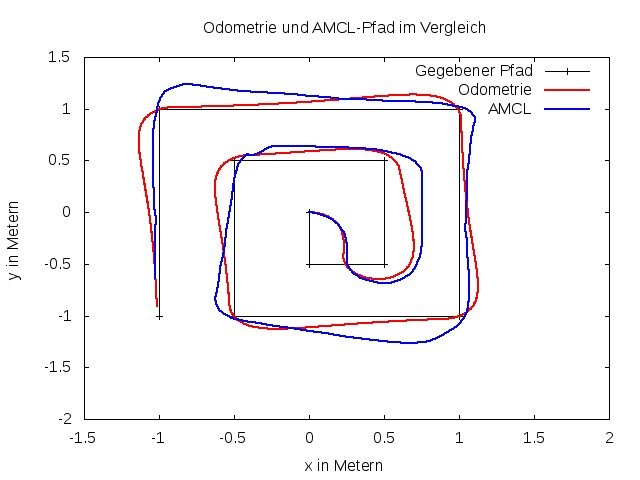
\includegraphics[width=0.45\textwidth]{pictures/path_odometry_slow.jpg}}
	\subcaptionbox{erh\"ohte Geschwindigkeit $\approx$ 3.2 m/s\label{fig:odoHighSpeed}}{
		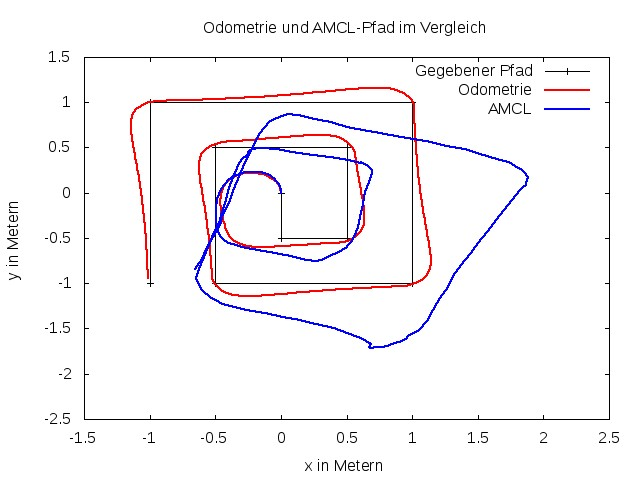
\includegraphics[width=0.45\textwidth]{pictures/path_odometry_fast.jpg}}
	\caption{Pfadverfolgung mit Odometrie}
\end{figure}

Zu beobachten ist, dass die Pfadverfolgung mit Odometrie bei geringer Geschwindigkeit ($\approx$ 0,714 m/s ) mit einer Abweichung von weniger als $\approx$ 30cm funktioniert. Siehe dazu Abbildung ~\ref{fig:odoLowSpeed}. Die Abweichung kommt dabei einerseits durch den \textit{Giovanni Controller} zustande, was auch bei der Simulation ersichtlich ist. Au{\ss}erdem ist die Odometrie fehlerbehaftet. Man erkennt zum Beispiel, dass der Roboter am Ende des Pfades etwa 30 cm zu wenig weit f\"ahrt.
Bei einer erh\"ohten Geschwindigkeit von $\approx$ 3.2 m/s folgt der Roboter dem Pfad deutlich schlechter siehte Abbildung \ref{fig:odoHighSpeed}. Dies liegt vermutlich daran, dass die R\"ader des Roboters vor allem in Kurven keinen Halt finden und durchdrehen.   

 

\begin{figure}[h]
	\centering
	\subcaptionbox{niedrige Geschwindigkeit $\approx$ 0,714m/s \label{fig:amclLowSpeed}}{
		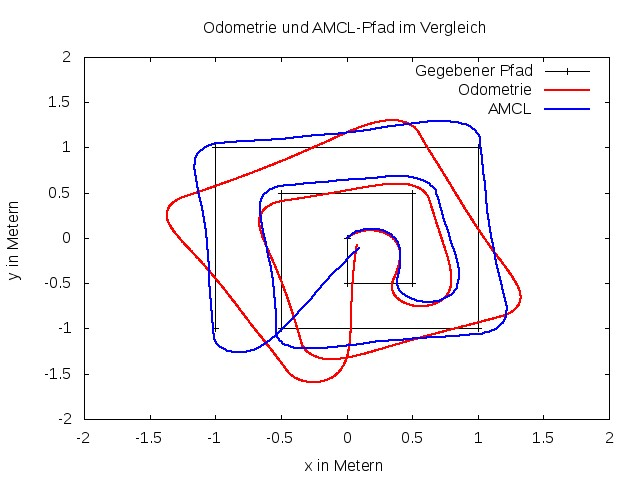
\includegraphics[width=0.45\textwidth]{pictures/path_amcl_slow.jpg}}
	\subcaptionbox{erh\"ohte Geschwindigkeit  $\approx$ 3.2 m/s \label{fig:amclHighSpeed}}{
		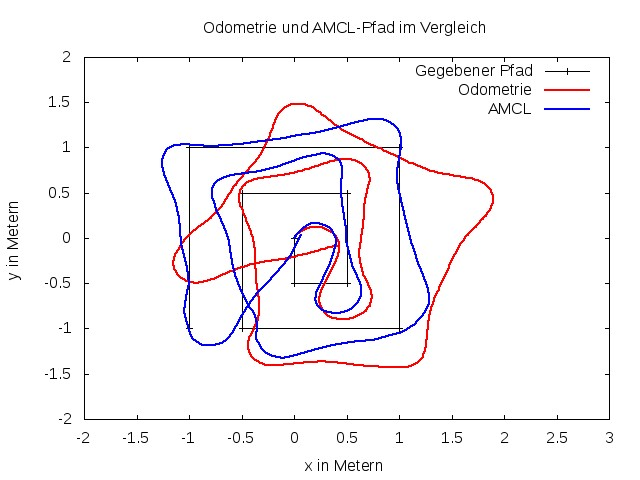
\includegraphics[width=0.45\textwidth]{pictures/path_amcl_fast.jpg}}
	\caption{Pfadverfolgung mit AMCL}
\end{figure}

Da bei \textit{AMCL} nicht \textit{AMCL} selbst als absolute Referenz verwendet werden kann, wird bei AMCL der Pfad zum Ausgangspunkt zur\"uck verl\"angert. In dem die Startposition auf dem Boden markiert wird, erkennt man die Pr\"azision mit der Roboter beziehungsweise der Algorithmus arbeitet.
Bei beiden Geschwindigkeiten erreicht der Roboter eine Genauigkeit von unter 20 cm. Der schneller abgefahrene Pfad weist geometrisch gr\"o{\ss}ere Abweichungen zum vorgegebenen Pfad auf. Der langsam abgefahrene Pfad hingegen schmiegt sich n\"aher an. Siehe dazu Abbildungen ~\ref{fig:amclLowSpeed} und ~\ref{fig:amclHighSpeed}.  
Dies liegt vermutlich daran, dass die Sample-Time von AMCL bei der erh\"ohten Geschwindigkeit  von $\approx$ 3.2 m/s nicht mehr ausreicht und so Abweichungen auftereten, bevor der Controller diese korregieren kann. 

\section{Zusammenfassung und Ausblick}

Dieses Paper pr\"asentiert einen Vergleich zwischen \textit{AMCL} und Odometrie, sowie Tests des \textit{Gmapping} Algorithmus und dem Pfadvefolgungsalgorithmus von Giovanni Indiveri. Die Tests wurden auf einer Roboterplattform mithilfe von \textit{ROS} durchgef\"uhrt. 


Dabei gab es keine \"uberraschenden Ergebnisse.

Die 2D-Kartierung einer unbekannten Umgebung erfolgt mittels \textit{gmapping} und liefert genaue Ergebnisse, wenn man die Hinweise im Abschnitt  \textit{Test von Gmapping}  beachtet.
Die Lokalisation mit Hilfe von Odometrie funktioniert schlechter als die mit AMCL, vor allem wenn der Roboter schnell f\"ahrt. Aber auch AMCL hat Schw\"achen und macht f\"ur Menschen sofort ersichtliche Fehler, siehe Abbildung  ~\ref{fig:amclFails}.
Lokalisierungsschwierigkeiten von \textit{AMCL} zeigen sich auch bei lautem Rauschen, zum Beispiel in Computerr\"aumen oder in R\"aumen ohne markante Anhaltspunkte. Bewegte Hindernisse wie Menschen werden zwar vom Laser erfasst, stellen aber bei der Kartierung keine Probleme dar und werden nicht in der Darstellung ber\"ucksichtigt. 

Der Roboter ist in der Lage selbst\"andig mittels Pfadverfolgung eine gegebene Punktewolke abzufahren. Die angegebene Punkte werden pr\"azise angesteuert, je dichter der Pfad in Punkten ausgedr\"uckt ist, desto genauer wird der Pfad verfolgt. Daraus l\"asst sich schlie{\ss}en, dass der Algorithmus des Giovanni Indiverdi korrekt funktioniert.

F\"ur die Zukunft kann die Odometriebestimmung verbessert werden, zum Beispiel beim Wechsel der Roboter durch Angabe pr\"azisere Reifengr\"o{\ss}en und Achsenl\"ange.
\\
Neuronale Netze erm\"oglichen durch pr\"azise Trainingsdaten einen Roboter auf verschiedene Situation vorzubereiten.


\section{Danksagung}
Die Autoren danken dem Hilfswissenschaftler Angel f\"ur die Unterst\"utzung und Hilfe bei verschiedenen Problemen mit dem Roboter und \textit{Robot Operating System}.
\\

{%\small                   % use small if you need it
	\bibliographystyle{plain}
	\bibliography{paper.bib}       % use a bib-file paper.bib to collect

}
\end{document}








